\documentclass[main.tex]{subfiles}
\begin{document}

On suppose que le modèle est soumis à des pertubations:
\[
  \begin{cases}
    \dot{x} = f(x) +g(x)u+p(x)w\\
    y = h(x)
  \end{cases}
\]
\begin{rem}
  Si $w$ modélise des incertitudes de modèle, alors on suppose que les erreurs de modélisation n'implique pas d'instabilité, $w$ ne dépend pas de $x$.
\end{rem}

On applique au modèle le principe du bouclage linéarisant:

\[
  y=h(x)=z_1\implies z_2\dot{z_1} = \dot{y} =h(x)
\]
Ainsi l'analyse sur le rejet de pertubation et réalisé sur la relation entre $r$ le degré relatif associé à $u$ et $\sigma$ le degré relatif associé à $w$.

\begin{itemize}
\item $r < \sigma$ : \\
  Alors le bouclage linéraisant a rendu la pertubation non commandable
\item $r \ge \sigma$:\\
  \begin{itemize}
  \item Soit on peux mesurer $w$ pour atténuer son effet
  \item Soit on modélise la pertubation, généralement sous forme canonique (ie $w^{(\alpha)}= 0$ , ou $\alpha$ est l'ordre). Pour avoir le cas $r<\sigma$ on réalise une observateur de pertubation et atténuer son effet.
\end{itemize}
\end{itemize}


\section{Rejet de pertubation via la commande par mode glissant}
\subsection{Exemple et Définitions}

Dans la commande par mode glissant on a $U = u_{eq}+u_y$ avec:
\begin{itemize}
\item $u_{eq}$ commande sans pertubation pour une poursuite asymptotique
\item $u_y$ commande à structure variable pour faire converger $x$ vers $x^*$.
\end{itemize}

\begin{exemple}
  Onduleur de tension commandé en courant


\newsavebox{\genericfilt}
\savebox{\genericfilt}{%
  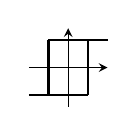
\begin{tikzpicture}[font=\small,>=stealth,scale=0.5]
    \draw[->] (-1,0)-- (1,0);
    \draw[->] (0,-1)--(0,1);
    \draw[thick] (-1,-0.7) -- (0.5,-0.7);
    \draw[thick] (1,0.7) -- (-0.5,0.7);
    \draw[thick] (0.5,-0.7) -- (0.5,0.7);
    \draw[thick] (-0.5,-0.7) --(-0.5,0.7);
  \end{tikzpicture}%
}
  \begin{figure}[H]\centering
  \begin{tikzpicture}
    \begin{scope}
      \begin{axis}
        [axis lines= middle,
        xmin= 0,xmax= 8,
        ymin =-2,ymax=2,domain=0:8,
        ]
        \addplot[no marks,blue,samples=200]{sin(deg(x))+0.1*sin(100*deg(x+1))};
        \addplot[no marks,red]{sin(deg(x))};
      \end{axis}
    \end{scope}
    \begin{scope}[shift={(7,3)}]
      \sbEntree{I}
      \sbComp{Comp}{I}
      \sbRelier[$i_{ref}$]{I}{Comp}
      \sbBlocL{N}{\usebox{\genericfilt}}{Comp}
      \sbSortie{Y}{N}
      \sbRelier[$y$]{N}{Y}
      \sbDecaleNoeudy[4]{Comp}{i}
      \sbRelier[$i$]{i}{Comp}
    \end{scope}
  \end{tikzpicture}
  \caption{Exemple de l'onduleur de tension}
\end{figure}

Si la fréquence est infinie on a un mode glissant
\end{exemple}


\begin{defin}
  Un système est à structure variable si la commande commute entre 2 valeurs suivant une logique $\sigma(x)$.
\end{defin}
\begin{prop}
  $\sigma(x)$ permet de glisser sur $S(x,t)$ surface de glissement si la fréquence de commutation est infinie. On a :
  \[
    V(x) = \frac{1}{2}S(x,t)^2 
  \]
  Soit :
  \[
    \dot{V}(x)= S(x,t)\dot{S}(x,t) <0 : \sigma(x)
  \]
\end{prop}
Dans un régime glissant on est dans un voisinage de $S(x,t)=0$ et pour maintenir le glissement la logique de commutation $\sigma(x)$ vérifie :
\[
  \lim_{S\to0^-} \dot{S} >0 \text{ et }\lim_{S\to0^+} \dot{S}>0
\]
\subsection{Application à la commande par mode glissant}

On utilise la méthode suivante
\begin{enumerate}
\item Choisir $S(x,t)$:
  Généralement $S(x,t)$ est obtneu par la porusuite asymptotique de $y$ (sortie du système) vers $y_c$, en choisissant une dynamique de poursuite linéaire. Alors on pose :$\epsilon(t)= y_c(t) -y(t)$ erreur de poursuite. et on a:
  \[
    S(x,t) = \epsilon^{(m)}(t)+\beta_{m-1}\epsilon^{(m-1)}(t)+ ... +\beta_1 \epsilon^{(1)}(t)+\beta_0 \epsilon(t)
  \]
  Avec $\beta_i$ tel que $p^m+\beta_{m_1}p^{m-1}+ ... \beta_0$ est un polynome d'hurwitz\footnote{Racine à partie Réelle négatives}.
  Généralement on prend :
  \[
    \left(
      \deriv[]{t}+\lambda
    \right)^m \epsilon(t)= 0 ,\lambda > 0
  \]
\item Trouver $u_g$ qui réalise la logique $\sigma(x)$ tel que $u_g = W signe(S)$, avec  $W> 0$. Ainsi on a :

  \[
    u = u_{eq}+u_g \text{ avec } \dot{S} = 0 \text{ pour } u_{eq}
  \]
\end{enumerate}

\subsection{Application au bouclage linéarisant}
On pose $m= r-1$ (où $r$ est le degré relatif) Alors on a :

\begin{align*}
  z_1 &= y = h(x) \\
  \dot{z_1} &= z_2 \\
 \dot{z_2} &= z_3 \\
           & \vdots \\
 \dot{z_r} &= v \\
\end{align*}
Avec
\[
  u  \frac{1}{L_gL_f^{r-1}}\left(
-L_f^r h(x)+\underbrace{y_c^{(r)}+\dot{S}+W.sgn(S)}_{v}
\right)
\]
Soit
\[
  v = y^{(r)}+\dot{S} + W sgn(S)
\]

À cette forme on rajoute une perturbation ( du au erreur du modèle):

\begin{align*}
  z_1 &= y = h(x) \\
  \dot{z_1} &= z_2 \\
 \dot{z_2} &= z_3 \\
           & \vdots \\
 \dot{z_r} &= y^{(r)} = v + \Delta  \\
\end{align*}
Avec $|\Delta| < K $. Pour assurer la poursuite de trajectoire on veux $ y^{(r)}=y_c^{(r)}$ Ainsi: $\dot{S} = - W sgn(S) -\Delta$. On pose $W = K \alpha$.
\begin{itemize}
\item Si $S > 0 \implies \dot{S} < -K (\alpha-1) < 0 \implies S\dot{S} <0 $ avec $\alpha >1$.
\item Si $S<0 \implies \dot{S} = W - \Delta > K(\alpha-1) >0 \implies S\dot{S} > 0 $
\end{itemize}


On a le mode de glissement avec $u_g = W sgn(S) $. C'est pour cette raison qu'on prend $W_{sat} =
\begin{cases}
  +U_{max}\\
  -U_{max}
\end{cases}
$
\subsection{Commande par mode glissant - Récapitulatif}

On fabrique la commande suivante pour rejeter les pertubations:
\[
  u = u_{eq} + u_g 
\]
où : 
\begin{itemize}
\item  $u_{eq}$ est la commande sans pertubation ni incertitude sur le modèle.
\item $u_g = W sgn(S)$  la fréquence de variation de $u_g$ doit être  très grande devant la dynamique de la poursuite.
\end{itemize}

Le problème de la discontinuité de $u$ dans les excitation des dynamiques du système. La solution est de réalisée la loi de commande sur $w= \dot{u}$, $u$ devient une variable d'état d'un\emph{ modèle augmenté}.

Sur le nouveau modèle on applique le mode glissant sur $w = w_{eq}+ w_g$

\end{document}
%%%Local Variables:
%%% mode: latex
%%% TeX-master: "main"
%%% End:
